\documentclass[compress,aspectratio=1610]{beamer}

\usepackage[ngerman]{babel}
\usepackage[english]{isodate}
\usepackage{amssymb}
\isodate
\usepackage{multicol}
\usepackage{tikz}
\usetikzlibrary{matrix,calc}
\usepackage{minted}

%% THEMES : vertex or green %%
%% OPTIONS: vertex & green %%
%%          [bincount] o. [bincount, totalframes]
%%          [hexcount] o. [hexcount, totalframes]
%%          []         o. [totalframes]
%% OPTIONS: vertex %%
%%          [dark] 
%%          [simplefootline]

%\usetheme[simplefootline, bincount]{vertex}
%\usetheme[totalframes]{green}
\usetheme[hexcount]{vertex}

\usepackage{blkarray}
\linespread{1.1}

\title{Veresterung}
\subtitle{Der Säurekatalysator}
\date{\today}
\author{Max Mustermann}
\institute[]{
  Fachhochschule Dortmund \\
  FB 10: Informationstechnik
}
\begin{document}

\maketitle

\section*{Inhalt}
\begin{frame}
  \frametitle{Inhalt}
  \centering
  \tableofcontents[hideallsubsections]
\end{frame}

\section{First Section}
\begin{frame}{Frametitle}
  \begin{block}{Aufzählungen}
    \begin{itemize}
    \item 1. Item
    \item 2. Item
    \item 3. Item
    \end{itemize}
  \end{block}
  \begin{block}{Zitieren}
    Wie in vorherigen Ansätzen \cite{Veresterung} \dots
  \end{block}
  \begin{block}{Math}
    $$f(x) = \sum\limits_{n=0}^{\infty}\frac{f^{(n)}(a)}{n!}x^n$$
  \end{block}
\end{frame}
\begin{frame}
  Your text here \dots
\end{frame}
\begin{frame}
  Your text here \dots
\end{frame}

\section{Bilder}
\begin{frame}{Frametitle II}
  \begin{figure}[!h]
    \centering
    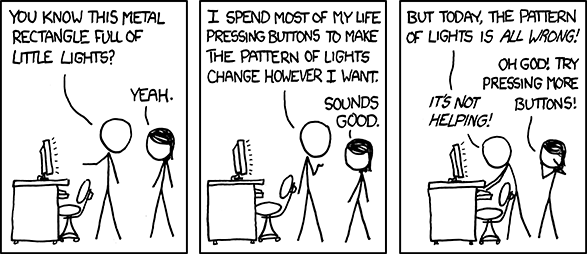
\includegraphics[width=0.7\textwidth]{figures/computer_problems.png}
  \end{figure}
\end{frame}
\begin{frame}
   Your text here \dots
\end{frame}
\begin{frame}
  Your text here \dots
\end{frame}

\begin{frame}{The End}
  \begin{center}
    Thank you for your attention, are there any questions?
  \end{center}
\end{frame}

\section*{The End}
\begin{frame}[allowframebreaks]
  \frametitle{Literaturverzeichnis}
  \bibliographystyle{ieeetr}
  \bibliography{literature.bib}
\end{frame}

\end{document}

